\section{Introdução}
\subsection{Ciência de dados}

De acordo com o \foreign{National Institute of Standards and Technology}\footnote{\url{nist.gov}}, ciência de dados (\foreign{data science}, DS) refere-se à atividade de extrair conhecimento acionável\footnote{Forma de saber científico que pode ser utilizada para a tomada de decisão.} de conjuntos de dados brutos utilizando processos de exploração ou formulação e teste de hipóteses.
Ela incorpora princípios, técnicas e métodos de diversas áreas, como ciências da computação, matemática e estatística, além de domínio da área de aplicação.

Essa área tem ganhado notorieade desde o início deste século devido ao crescimento exponencial na geração de dados, conhecido genericamente como \foreign{Big Data}, devido principalmente ao advento da Web 2.0, por volta de 2005, e dos dispositivos móveis, em 2007.
Desde então e também devido ao aumento na capacidade computacional, novas técnicas de análise, a maioria computacionais, tem sido empregadas.
Exemplos notáveis são as redes neurais e a inferência bayesiana.

Mais recentemente, inúmeras ferramentas robustas de computação e análise de dados, disponibilizadas livremente, tem tornado a ciência de dados cada vez mais acessível.
Exemplos são as linguagens de programação Scala, Python (e suas bibliotecas de análise de dados), R e, mais recentemente, Julia.
Isso sem mencionar a abordagem AutoML, que oferece interfaces simples para o emprego de aprendizagem de máquina sem a necessidade de programação.

A facilidade de acesso e a alta demanda por cientistas de dados levou, então, à oferta de cursos de ciência de dados \cite{Hassan2019}:\footnote{Veja \url{kdnuggets.com/education/usa-canada.html}} no Brasil, algumas universidades já oferecem graduações (\eg, Univesp) e pós-graduações (Instituto de Ensino Insper), mas também é possível estudar gratuitamente pela Internet, nas plataformas MOOC (\foreign{massive open online courses}) como Coursera, EdX \etc.

Há também cursos livres nessa área (\eg, Digital House e Tera), que ganham força devido ao reconhecimento de que as universidades tradicionais já não suprem a necessidade de mão de obra qualificada em várias áreas \cite{Zulauf2006}.
Esses cursos oferecem uma formação rápida, de alguns meses, capaz de colocar o candidato no mercado de trabalho, independentemente da sua área de formação.

\begin{figure}
	\centering

	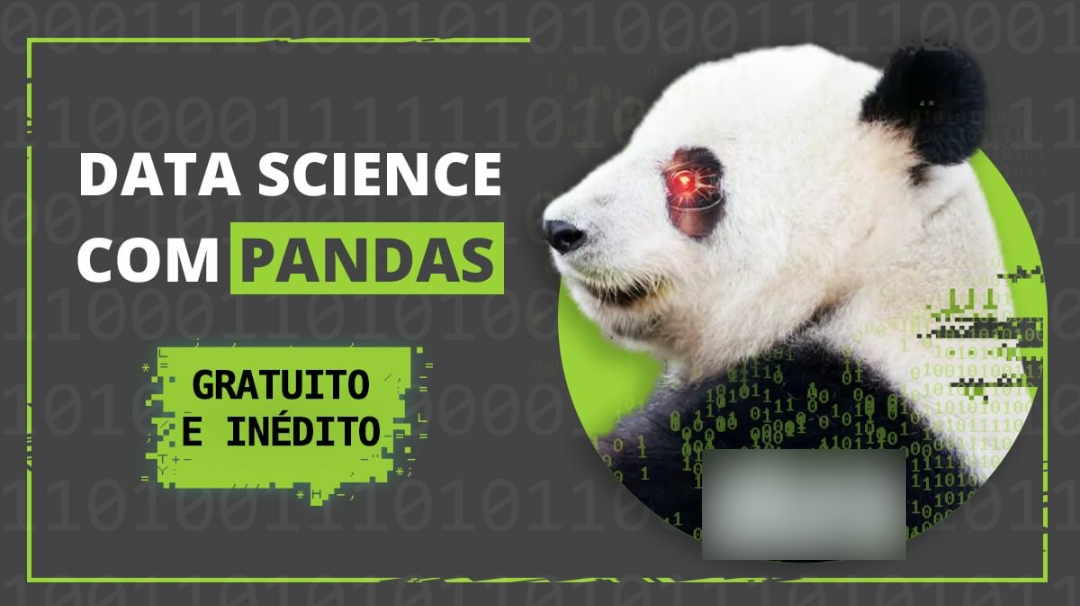
\includegraphics[width=0.45\textwidth]{eg_ds_1}\hfill
	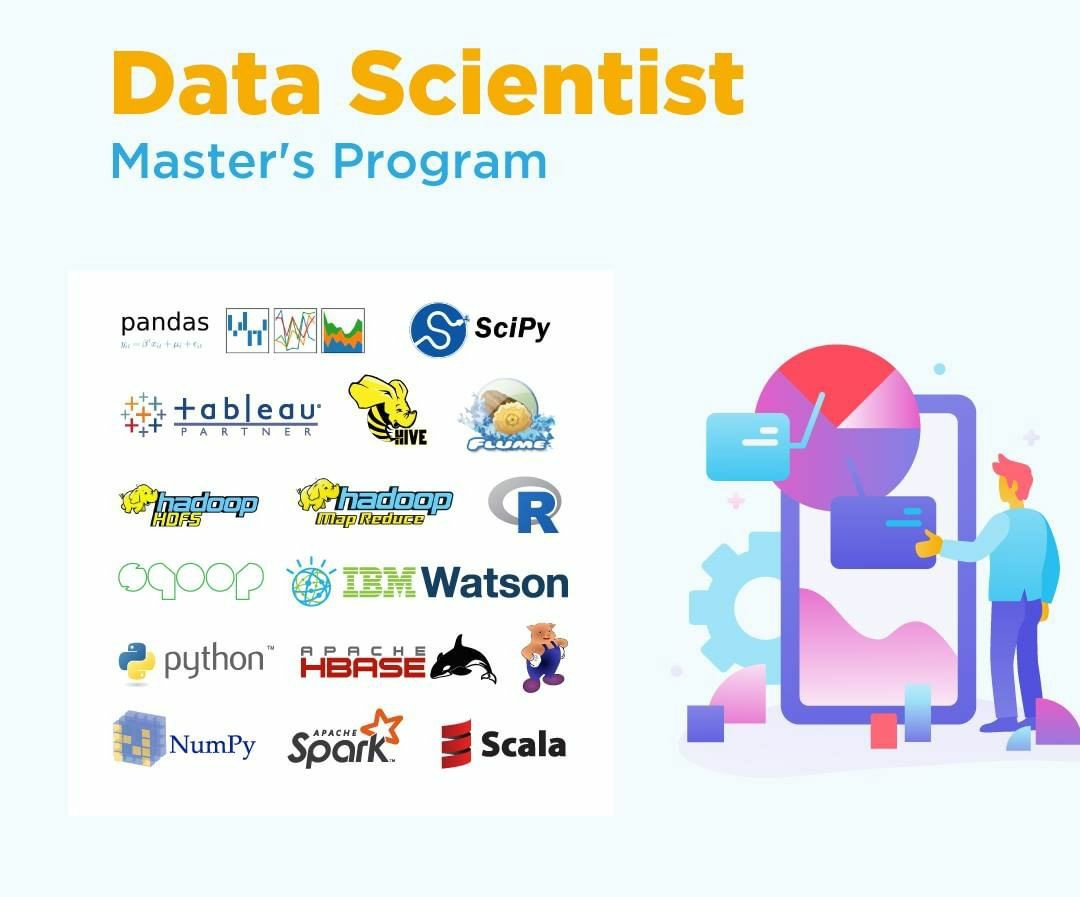
\includegraphics[width=0.45\textwidth]{eg_ds_2}

	\caption{Em geral, cursos livres de ciências de dados enfatizam a utilização de aplicativos, linguagens de programação e algoritmos ao invés de competências e habilidades necessária.}
	\label{fig:cursos}
\end{figure}

Porém, como esses cursos visam o mercado de trabalho, em geral eles enfatizam não os conhecimentos, competências e habilidades que um cientista de dados precisa, mas as ferramentas e algoritmos requeridos pelas vagas de emprego.
A figura~\ref{fig:cursos} ilustra isso: ela apresenta a propaganda de dois cursos, oferecidos na rede social Instagram.
Em ambos a proposta concentra-se em linguagens de programação (Python, Scala e R), ferramentas de \foreign{Big Data} (Spark, Hadoop \etc), aplicativos (Tableau) e bibliotecas (Pandas, SciPy \etc).

Embora o domínio dessas ferramentas seja necessário, elas não são suficientes para um cientista de dados de fato obter conhecimento acionável.
Para isso são necessários, por exemplo, métodos de pesquisa, engenharia de dados, inferência estatística, dentre outros \cite[p.~15]{CF-DS-Release2019}.

\subsection{Competências e habilidades}

No Brasil e no mundo, a proposta de substituir os currículos tradicionalmente baseados em conteúdo por aqueles baseados em competências e habilidades tem ganhado força: por exemplo, veja a Base Nacional Comum Curricular\footnote{Acesse \texttt{basenacionalcomum.mec.gov.br}.} (BNCC) brasileira ou \cite{Inkson2017}, na Austrália.

Essa abordagem tem sido adotada no ensino básico \cite{Avila2017} e superior\footnote{\url{eletroensino.blogspot.com/2013/02/formacao-baseada-em-competencias-no.html}} para direcionar a ``educação brasileira para a formação humana integral e para a construção de uma sociedade justa, democrática e inclusiva''.
De fato, essa abordagem visa a empregabilidade \cite{Voorhees2001}, que é também o objetivo dos cursos livres anteriormente mencionados.


Entretanto, as vagas de trabalho em ciências de dados frequentemente apresentam como requisitos as ferramentas e algoritmos anteriormente mencionados ao invés das competências e habilidades necessárias para o exercício da ciência de dados.
A figura~\ref{fig:vagas} ilustra duas vagas dessa área, obtidas na plataforma LinkedIn.
Nela podemos ver a menção às mesmas ferramentas e algoritmos oferecidos pelos cursos livres.

\begin{figure}
	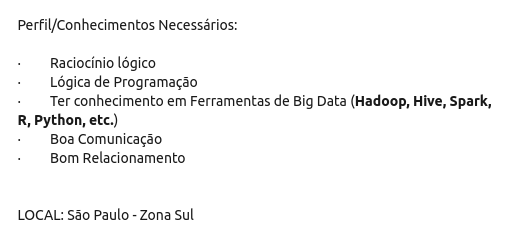
\includegraphics[width=0.45\textwidth]{eg_vaga-1_ds}\hfill
	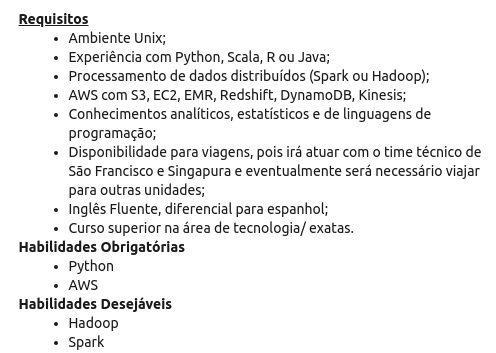
\includegraphics[width=0.45\textwidth]{eg_vaga-2_ds}
	\caption{Duas vagas de cientista de dados, extraídas do LinkedIn.}
	\label{fig:vagas}
\end{figure}

\subsection{Cenário e motivação}

Em vista do exposto, o autor deste trabalho, que atua como coordenador numa instituição educacional que oferece cursos livres de DS e \foreign{data analytics} (DA), gostaria de adotar a aprendizagem baseada em competências (seção \ref{sec:competencias}) nos cursos de ciência de dados e de \foreign{data analytics} (DA) sob sua responsabilidade.

Neste trabalho nós analisamos os resultados de aprendizagem nos cursos de DA e DS oferecidos pela instituição educacional mencionada, com o intuito de identificar uma possível concorrência entre os currículos baseados em competências e os incentivos do mercado de trabalho, conforme exposto nas hipóteses deste trabalho (seção~\ref{sec:hipóteses}).

Conforme a definição de ciência de dados do NIST, os cursos de DA e DS podem ser classificados como de ciência de dados.
Porém, eles guardam semelhanças e diferenças entre si:
\begin{compactdesc}
	\item[\foreign{Data Analytics} (DA):] visa a inteligência de mercado (\foreign{business intelligence}, BI), isto é, a aplicação da ciência de dados para obter conhecimento acionável que suporte decisões estratégicas para um empreendimento.
	Esse curso tem carga-horária de 140 horas e dura 14 semanas.
	Outra característica desse curso é que ele baseia-se em aplicativos como PowerBI, Tableau, MySQL \etc.

	\item[\foreign{Data Science} (DS):] visa o desenvolvimento de ``produtos de dados'', \ie, \foreign{softwares} que automaticamente obtém conhecimento acionável para oferecê-lo aos clientes.
	Esse curso tem carga-horária de 196 horas, dura 19 semanas e baseia-se na linguagem de programação Python e suas extensões para análise de dados.
\end{compactdesc}